
\section{Evolving the SPL Conceptual Architecture}
\label{sec:spl_project}

The SPL conceptual architecture (Figure \ref{fig:schema}) was evaluated by 31 participants from different areas of expertise, considering the stakeholders' perspective \cite{marcolinoarcht2017}. Based on their profiles, we noticed that all of them are from academic area, implying in a possible bias in the evaluation of the architecture in a industry perspective.

Other issue refers to the results related with \textit{conceptual aspects}, \textit{infrastructure aspects} and \textit{SOA aspects}. Comparing the results with the \textit{general aspects} and \textit{educational domain aspects}, the percentage of results that ranked the architecture as \textit{partially complies} suggests possible issues to be reanalyzed. 

It was also identified the need of evaluating the architecture and the requirements catalog together, since they had been evaluated separately, what could imply on issues such as imprecise understanding of the software solutions. If the \textit{domain design} and \textit{domain realization} SPLE sub-processes are conducted without proper analysis, the cost and effort to re-factor the project and the sub-processes involved could be higher. Thereby, a reevaluation of the proposed architecture was conducted.


\subsection{Methodology}

The methodology applied to support the new analysis of the conceptual architecture follows an industry protocol in which the requirements and needs were deeply analyzed for proposing the architecture.

Such industry protocol involves the process of rigorous analysis of (i) each requirement (functional and non - functional) independently, for the identification of it possible impact and development technique to be adopted; (i) the analysis of set of requirements and possible expect and unexpected behaviors, when combined with other sets of requirements; (ii) architectural designing decisions for each set of requirements and after, for the entire solution; (iv) technical debt issues and; (v) human resources available in the development team and time.

Then the following steps were conducted:

\begin{itemize}
\item the previous architecture model (Figure \ref{fig:schema}) and its publication were analyzed;
\item the requirements catalog was discussed considering the ideas of the first architecture model and the learning and didactic objectives to minimize problems \cite{souza2015} in programming domain considering mobile learning applications; and
\item based on the previous analysis, each package/layer in the conceptual architecture was studied and restructured when necessary.
\end{itemize}

The analysis occurred during one month, where two practitioners from the industry supported the evolution of the model. Both have an average of eight years of expertise in mobile development in industry. One of them have also expertise in software product line, three years, and the other one in development of hybrid applications, five years.

It is highlighted that the number of practitioners is small, but considering the availability and the reality of Brazilian academy agreements with software industries, this interaction, even in with a small participants, allows the identification of possible lack of know-how in academic perspective, where the theoretical knowledge is bigger than the practice. Finally, it is also emphasized that the participants also collaborate with the development of the UML models with SMarty.

\subsection{Discussions and Evolved Conceptual Architecture}

After the execution of each step previously discussed, the conceptual model was updated as shows Figure \ref{fig:schema2}.


\begin{figure*}[!ht]
    \centering
    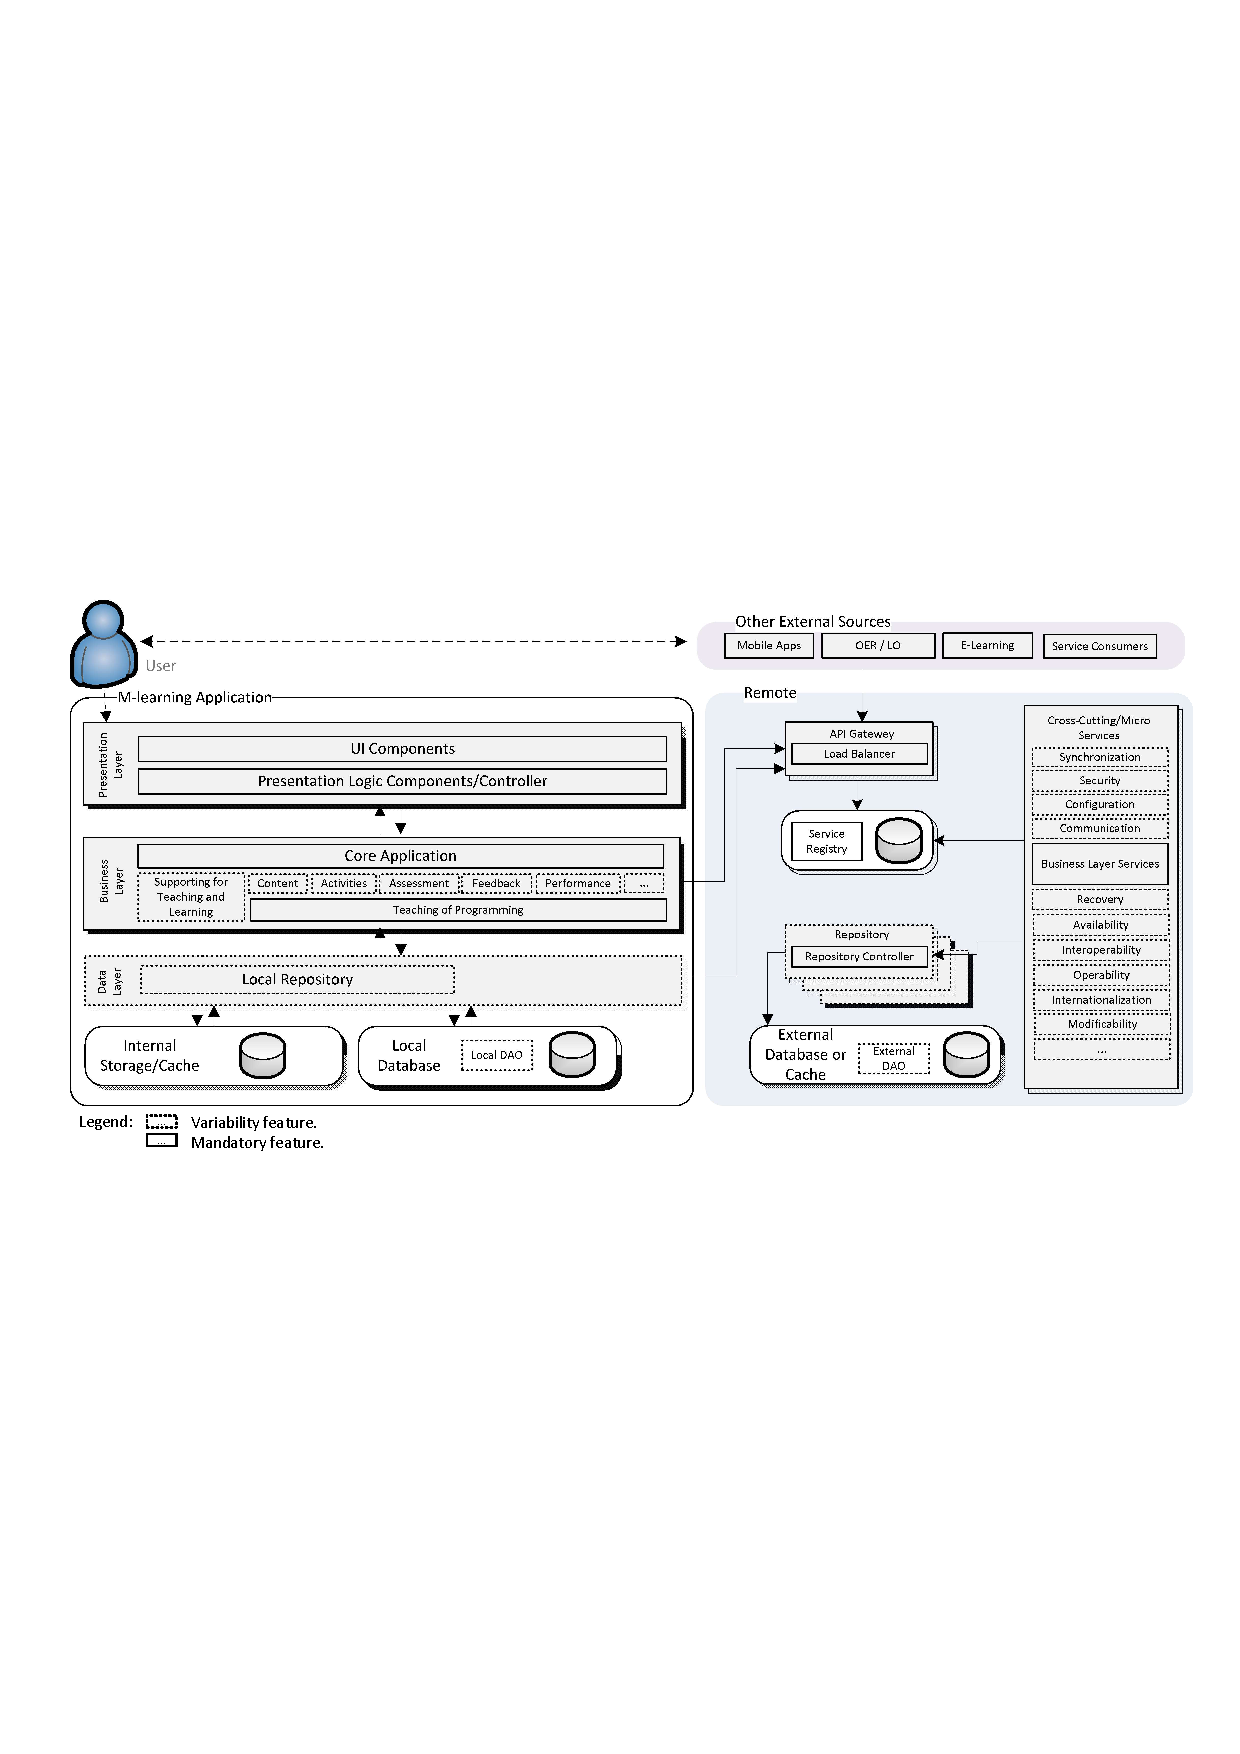
\includegraphics[scale=0.90]{archv7.pdf}
    \caption{Updated M-learning SPL Conceptual Architecture.}
    \label{fig:schema2}
\end{figure*}

\textit{Domain Engineering}, \textit{Application Mechanism} and \textit{Application Engineering} do not changed (Figure \ref{fig:schema}). All of them continue with the same roles and sub--processes, with the exception from the way in which the applications are generated. This change implies in most of the changes in the m--learning application architecture.

For the user, the \textit{application mechanism}\cite{marcolinoarcht2017} will work in the same way: the user answers some questions or selects the desired features and the support mechanism generates the application for download. However, with the updates, the choices made by the users will be stored in a database (or metadata files) and will be considered for delivering an application instantiated with only the selected features. So, if the institution privilege is considered, only a set of features allowed for it will be available for the users' institution. This software architecture strategy is called multi--tenancy.

The mult--tenancy architecture refers to an architecture in which a single software solution is executing on a server, serving multiple groups of users who share common access in such instance of software. Each of these groups is called tenant. Looking at cloud computing models, the multi--tenancy approach is perfectly adherent to Software as a Service (SaaS) \cite{krebs2012architectural}.

The change in the application mechanism implies in a delivery of a complete application instance (presentation and business layers), no matter the selected features. However, at the end, the application will solve its variabilities in execution time based on the set of selected features, providing only features and services related to the current user, the owner of the configuration defined in advance.

In the multi--tenancy proposal, the code and database packages are installed on a single server, simplifying the release and scalability processes \cite{krebs2012architectural}.

At this point, many concerns arise:


\textbf{Q1 -- Why was this decision made?}

Imagine the hypothetical scenario where a teacher generated an application for two classes to be used in one semester. After finished the period, he receives in the next semester four more classes, but now he wants to use the application with a new feature, not selected in the previously semester. Until now there is no problem. He can generate another application and use it with his new classes but, and the data from the other application? Additionally, if the teacher decides to change his choices for the application in the middle of semester, he will need to create a new application and re--install each student's application. Furthermore, if the new configuration is not concise with the previous features -- in a software product line constraint perspective -- teachers and their students will not be able to correctly use the application with the new changes. 

A final issue is the number of applications to be controlled based on several teachers and classes in the same institution. Data for the educational administrator will be always broken in parts, making the process to manage and to improve the learning and teaching processes difficult, mainly by each specificity of the applications. It is highlighted that this requirement was not change, just new considerations were made, allowing a deeper understanding of the features, besides, this is only one of several implications that were identified, leading to the proposed changes.




\textbf{Q2 -- Do these changes not imply in significantly changes on the functionality of the applications?}

Yes, mainly about the connection-dependency. Adopting multi--tenancy implies in a connection, since this connection will be required for the presentation layer shows only the features selected for the current user. However, cache and local database can be used to allow the use of the application when a connection is not available, mainly when a mobile device is the platform in use. Such usage is the reason for a new update in the architecture: the adoption of repository pattern, later discussed in this section.

\textbf{Q3 -- Which trade-off may these types of application have?}

\begin{itemize}


\item \textbf{Positive factors:} one instance in a server for multiple users, centralizing scalability issues and simplifying the release management.

\item \textbf{Negative factors:} Larger development effort, mainly to maintain and to use per--tenant data allowing the customization of the applications. Furthermore, multi--tenancy increases the risks and impacts inherent in applying a new release version. As there is a single software instance serving multiple tenants, an update on this instance may cause downtime for all tenants even if the update is requested and useful for only one tenant \cite{krebs2012architectural}.

\end{itemize}

%There are other positive and negative factors but those are highlighted considering its integration in an SPL for the development of mobile learning applications in a fist instance.

Based on the adoption of multi--tenancy, a new challenge appears: guarantee the correct execution of applications in mobile devices in areas where network connection is not available. For this, as mentioned in \textbf{Q2}, the repository pattern was adopted as a solution in the SPL architecture proposed. Although, before the understanding of this pattern, it is important to make an observation related to the pedagogical and didactic concern: the constantly feedback in applications.

According to Marcolino and Barbosa \cite{marcolinoarcht2017}, there is a problem in the given feedback in mobile applications for the teaching of programming. As such applications generally support informal than formal learning, feedback features are given only for one of the categories of the users, teachers or students. Thereby, the need of a more concise feedback to support students to learn by themselves and to notify teachers about the students' performance is a mandatory pedagogical and didactic feature to support formal learning. The feedback allows the improvement of the curricula, changes on didactic strategies adopted in classroom, changing on teaching topics and other improvements \cite{marcolino_catalog2016}. Thus, the adoption of a mechanism to store and retrieve the data of the learning process is fundamental, meeting the need for the adoption of mechanisms to enable it, as the repository pattern does.

The repository pattern avoid the directly access of data from the business logic layer, services or other entities, reducing the duplicate code, weak types of business data, the difficulty in centralizing data from cache and several data bases and, the inability to easily test the business logic \cite{repository}. The pattern manages several data repositories, common in a microservices architecture and it also enables caching and storing data in mobile applications. Based on these benefits, the repository pattern was selected to deal with the multi--tenancy concerns, integrating a DAO (data access object) strategy when convenient, and easing the manage of data from the microservices -- other update in the proposed SPL architecture.

The repository is shown in Figure \ref{fig:schema2}. It is available in two perspectives, directly in the client application or in the server side. The \textit{local repository} can realize the persistence through internal storage, i.e., private data in the device memory; or in local database, i.e., structured data in private database and; with network connection, i.e., calling a microservice. On the other hand, the repository on the server side is used by the microservices only, and realize its persistence through a external storage, i.e., a database or cache \cite{repository}.

Among other benefits encompassed with the adoption of the repository pattern, we highlight that: (i) they can adopted different persistence strategies for different contexts, such as relational databases, non-relational databases, cache and services; and (ii) applications can adopt managers for easing the integration and encapsulation of the dependencies strategies.


Finally, the last update made was the adoption of microservices concept, which integrates the SPL proposal for the development of applications as a SaaS \cite{Newman:2015:BM:2904388}. 

The adoption of mobile learning applications has several benefits (see Section \ref{sec:background}). However, the management of data, the availability of new content, learning activities and other elements presented in a learning environment though the reduced mobile screens and its native keyboard may not be a good way for conducting such tasks. In this perspective, providing different paths of access to those functionalities in different platforms can improve the user experience and, microservices support this strategy.


\begin{figure*}[!ht]
    \centering
    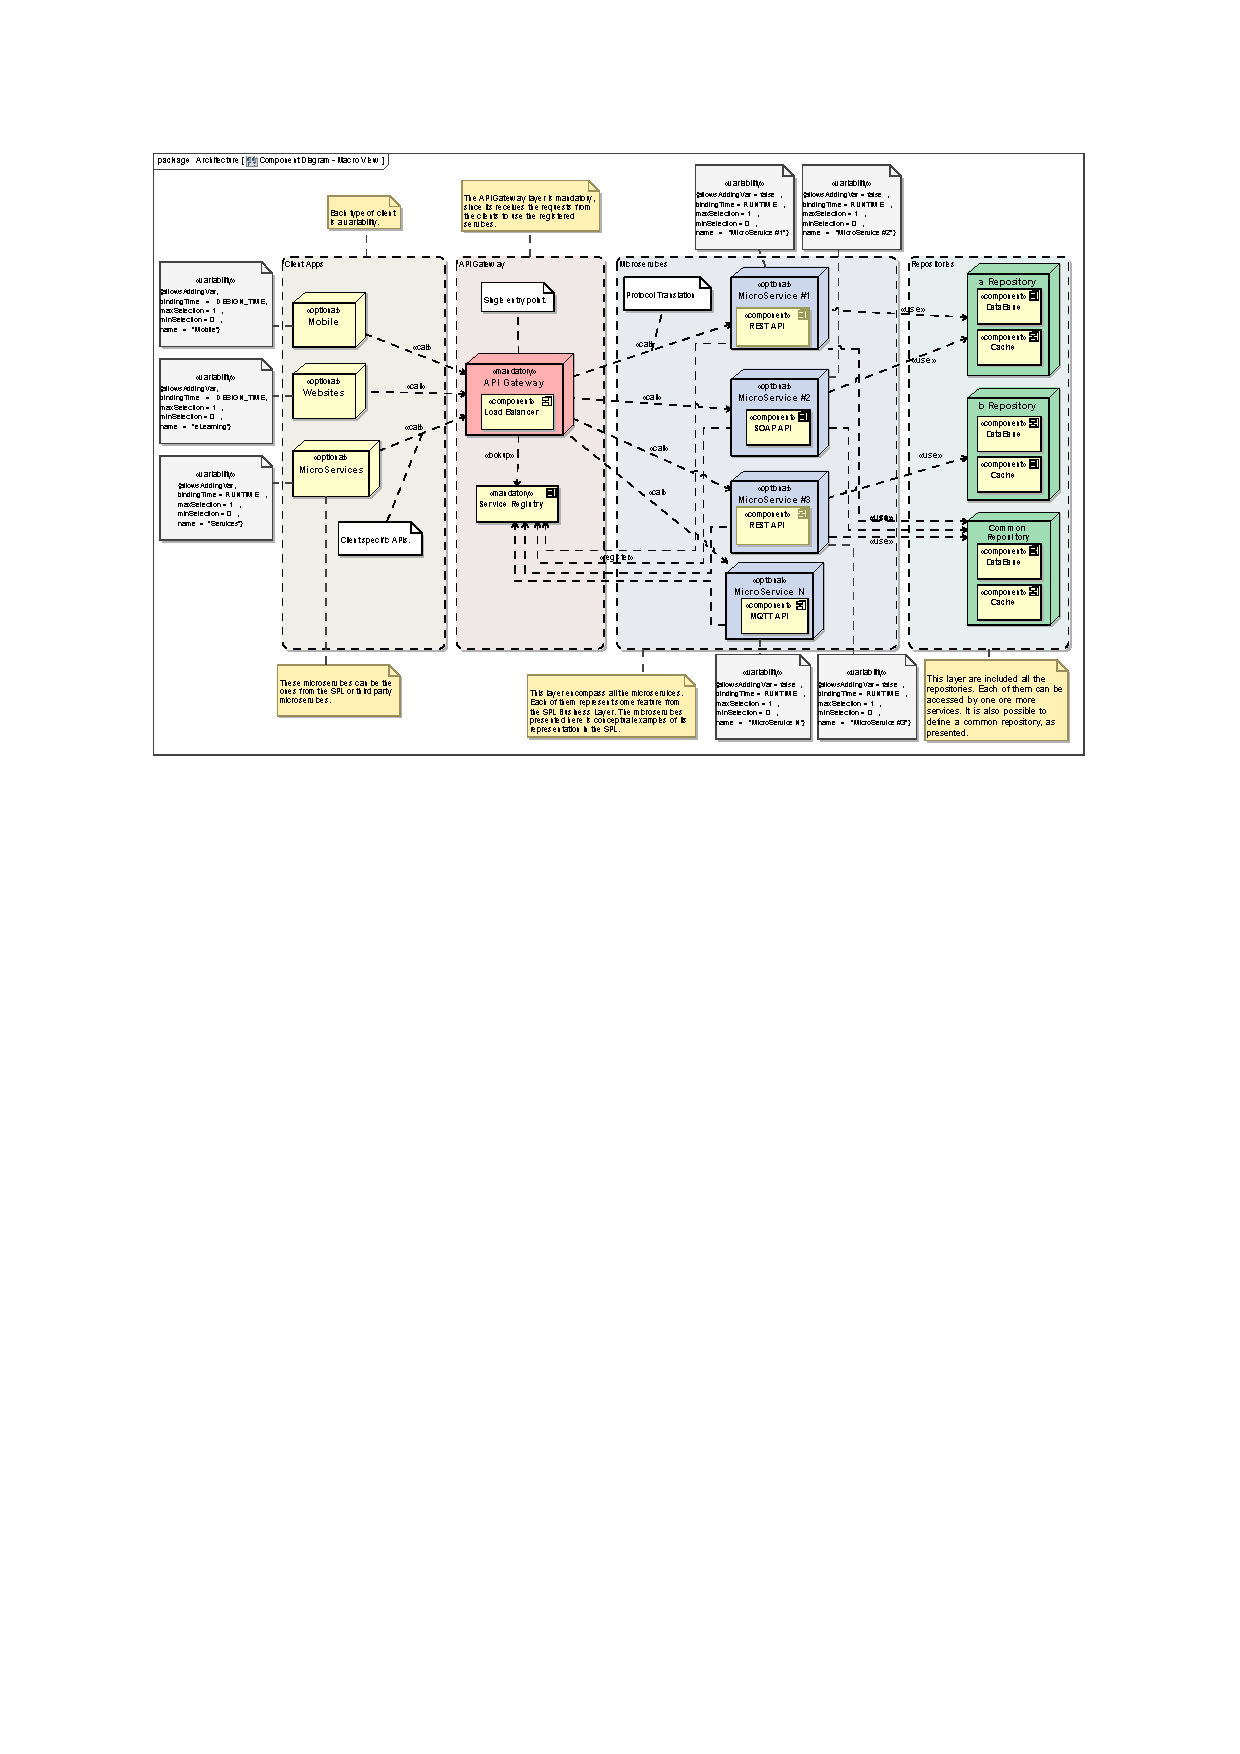
\includegraphics[scale=1.00]{component.pdf}
    \caption{M-learning SPL Component Model.}
    \label{fig:comp}
\end{figure*}

Microservices allow the use of different platforms and technologies as consumers of them. The responsibility is uncoupled from the business layer, which has only the function of accessing the microservices available on one or more servers and providing for the presentation layer such functionality. Looking at the SPL concept, the microservices meet and facilitates the process of management and definition of variabilities. Microservices provide a set of fully uncoupled services, but highly collaborative. Each service implements a set of narrowly, related functions. For example, an application might consist of services such as the order management service, the customer management service, etc.

Services communicate using either synchronous protocols, such as HTTP/REST (Representational state transfer), SOAP (Simple Object Access Protocol), or asynchronous protocols, such as AMQP (Advanced Message Queuing Protocol) and MQTT (Message Queue Telemetry Transport). Also, they can be developed and deployed independently of one another \cite{Newman:2015:BM:2904388}. As each service has its own database, the data consistency is improved. Add a data management standard, such as repository, and you'll have an even more robust solution. And, considering the multi-tenancy architecture, just the features selected in advance will be available and visible for each tenant/user.

Also in Figure \ ref {fig: schema2}, other difference from the first model is clear: the relation between \textit{other external sources} with the application. This goes to meet what was discussed about the multi--tenancy and microservices. These external sources will benefit from these adoptions, since its relation with the \textit{API Gateway}, its \textit{load balancer} and the \textit{service library} will allow the consumption of the microservices by other platforms or even by other applications, improving the reuse of features not dependent from the domain of the line.

The extra \textit{service layer} was removed and the \textit{core application} component replaced the \textit{application facade/interface}. Now, the \textit{business layer} has a relation with the \textit{API Gateway}, which balances the requests among the different tenants and applications to the microservices which are, in their turn, registered in a data base managed by the \textit{service registry}. Every microservice that reflects a feature in the SPL and is available to be selected by users, has a register entry that is visible by the \textit{service registry} and available by it for the \textit{API Gateway}, responsible to redirect each requisition received from the \textit{business layer} or \textit{external sources} for its respective microservice.

Among other benefits encompassed with the adoption of microservices, we highlight that: (i) they are independent; if one fails or goes to maintenance, the others will continue available; (ii) they can be implemented adopting different technologies; (iii) they can have one or more repositories; and (iv) they can be encapsulated and works only with the complexity from the business domain, easing the development, since the complexity is distributed among such domains.

Some concerns also emerged with its adoption: (i) it is hard to separate business domains, but for our SPL this difficulty does not occur, since the mentioned m-learning requirements catalog solve this concern; and (ii) the deploy of several microservices and the hardware maintenance need more efforts than the development of monolithic systems.


We also highlight some API Gateway benefits: (i) it is adopted as a facade layer with the objective to facilitate the clients' accesses to the microservices; and
(ii) it is an ``intelligent'' layer that can balance the load of number of requisitions and the caching information.
 
On the other hand, one concern is the disadvantage in the creation of a single point of failure.



Therefore, with the macro view of the conceptual SPL architecture updated, the \textit{domain design} sub-process is retaken Its artifacts models are presented and discussed next.

